\textbf{Analyze \#1:} \newline
\phantom{ } We built the circuit according to the lab instruction, and recorded the following data.\\
\begin{table}[!htbp]
	\centering
	\caption{Amplitude and phase change of output signal of preamplifier}
	\begin{tabular}{lccccc}
		\toprule
		No &freq($\si{\hertz}$) &Amp\_in($\si{\milli\volt}$)&Amp\_out($\si{\volt}$)&Phase&gain(dB)\\
		\midrule
		1	&10		&104	&4.6	&180.00	&32.9145\\
		2	&20		&104	&4.6	&178.56	&32.9145\\
		3	&50		&108	&4.6	&183.60	&32.5867\\
		4	&100	&104	&4.6	&174.24	&32.9145\\
		5	&200	&106	&4.6	&178.56	&32.7490\\
		6	&500	&104	&4.6	&180.00	&32.9145\\
		7	&1000	&108	&4.9	&175.68	&33.1355\\
		8	&2000	&108	&4.9	&172.80	&33.1355\\
		9	&5000	&110	&4.7	&162.00	&32.6141\\
		\bottomrule
	\end{tabular}
	\label{tab:preamp}
\end{table}
\phantom{ } Then we plot the Bode plot in Excel according to table[\ref{tab:preamp}] in figure[\ref{fig:101},\ref{fig:102}].

\begin{figure}[!htbp]
	\centering 
	\begin{framed}
		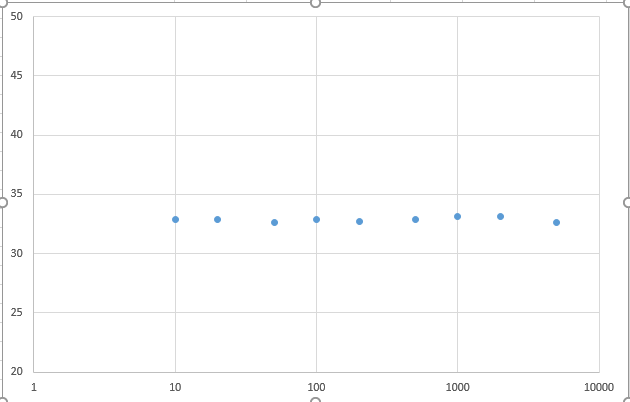
\includegraphics[width=\linewidth]{images/1_1.PNG} 
		\caption{Bode plot of preamplifier(y:gain(dB),x:frequency(Hz))}
		\label{fig:101} 
	\end{framed}
\end{figure} 

\begin{figure}[!htbp]
	\centering 
	\begin{framed}
		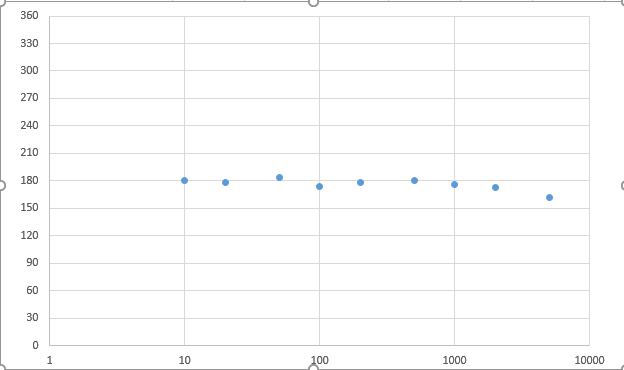
\includegraphics[width=\linewidth]{images/1_2.PNG} 
		\caption{Bode plot of preamplifier(y:phase,x:frequency(Hz))}
		\label{fig:102} 
	\end{framed}
\end{figure}

\phantom{ } We can see that the gain and phase change remains a similar value compared to the prelab result. When the frequency gets to 5000Hz, both gain and phase change falls down a little, which meets the result in prelab.

\phantom{ } We then change the amplitude and frequency of the input signal to 300mV and 300Hz. The waveform on the oscilloscope is shown in figure[\ref{fig:103}]. We can see that the phase change stays at $ 180^{\circ} $, and the gain is also a constant. We can also see that the output waveform distorted at the peak and the bottom to a flat figure. We think the reason is that the gain and input amplitude makes the output amplitude reaches the source voltage, thus the output amplitude won't go higher or lower.\\
\begin{figure}[!htbp]
	\centering 
	\begin{framed}
		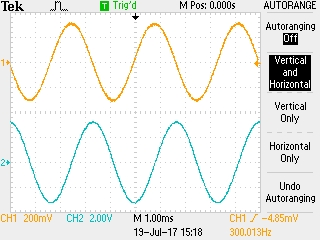
\includegraphics[width=\linewidth]{images/osc1.png}
		\caption{Waveform of the integrator}
		\label{fig:103} 
	\end{framed}
\end{figure} 

\textbf{Analyze \#2:} \newline
\phantom{ } After setting the resistance of the potentiometer to 50$ \si{\kilo\Omega} $, we recorded the following data.
\begin{table}[!htbp]
	\centering
	\caption{Amplitude and phase change of output signal of preamplifier(with 50$ \si{\kilo\Omega} $)}
	\begin{tabular}{lccccc}
		\toprule
		No &freq($\si{\hertz}$) &Amp\_in($\si{\milli\volt}$)&Amp\_out($\si{\volt}$)&Phase&gain(dB)\\
		\midrule
		1	&10		&108	&9.4	&172.80	&38.7941\\
		2	&20		&108	&9.4	&177.12	&38.7941\\
		3	&50		&106	&9.4	&178.20	&38.9564\\
		4	&100	&106	&9.4	&177.12	&38.9564\\
		5	&200	&106	&9.4	&178.56	&38.9564\\
		6	&500	&106	&9.4	&174.60	&38.9564\\
		7	&1000	&108	&10		&175.68	&39.3315\\
		8	&2000	&110	&9.8	&165.60	&38.9967\\
		9	&5000	&112	&8.8	&145.80	&37.9053\\
		\bottomrule
	\end{tabular}
	\label{tab:preamp50}
\end{table}

\phantom{ } Then we plot the Bode plot in Excel according to table[\ref{tab:preamp50}] in figure[\ref{fig:104},\ref{fig:105}].
\begin{figure}[!htbp]
	\centering 
	\begin{framed}
		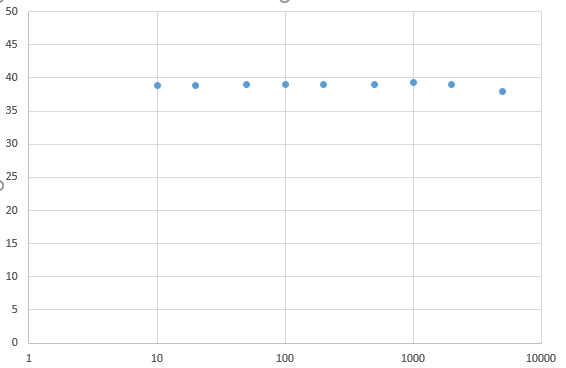
\includegraphics[width=\linewidth]{images/1_3.PNG} 
		\caption{Bode plot of preamplifier(50$ \si{\kilo\Omega} $)(y:gain(dB),x:frequency(Hz))}
		\label{fig:104} 
	\end{framed}
\end{figure} 

\begin{figure}[!htbp]
	\centering 
	\begin{framed}
		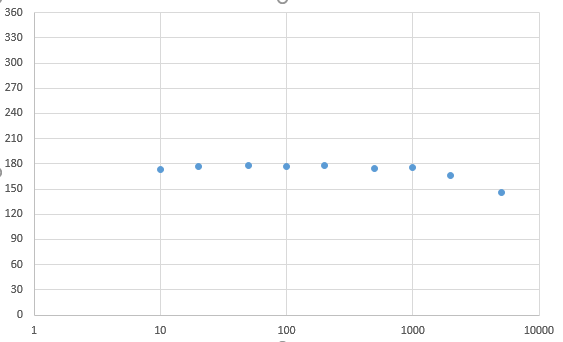
\includegraphics[width=\linewidth]{images/1_4.PNG} 
		\caption{Bode plot of preamplifier(50$ \si{\kilo\Omega} $)(y:phase,x:frequency(Hz))}
		\label{fig:105} 
	\end{framed}
\end{figure}

\phantom{ } We can see that in the gain is higher than the one in analysis \#1. Also, the phase change is lower and falls more quickly than in analysis \#1. We can see that the potentiometer brings the preamplifier a higher gain and a lower phase change.\\

\textbf{Analyze \#3:} \newline
\phantom{ } Then we built a summing amplifier according to the lab instruction, and set the correct amplitude of the input signal, then we recorded the following data.

\begin{table}[!htbp]
	\centering
	\caption{Amplitude and phase change of output signal of summing amplifier}
	\begin{tabular}{lccccc}
		\toprule
		No &freq($\si{\hertz}$) &Amp\_in($\si{\milli\volt}$)&Amp\_out($\si{\volt}$)&Phase&gain(dB)\\
		\midrule
		1	&10		&108	&9.4	&172.80	&38.7941\\
		2	&20		&108	&9.4	&177.12	&38.7941\\
		3	&50		&106	&9.4	&178.20	&38.9564\\
		4	&100	&106	&9.4	&177.12	&38.9564\\
		5	&200	&106	&9.4	&178.56	&38.9564\\
		6	&500	&106	&9.4	&174.60	&38.9564\\
		7	&1000	&108	&10		&175.68	&39.3315\\
		8	&2000	&110	&9.8	&165.60	&38.9967\\
		9	&5000	&112	&8.8	&145.80	&37.9053\\
		\bottomrule
	\end{tabular}
	\label{tab:sumamp}
\end{table}

\phantom{ } Then we plot the Bode plot in Excel according to table[\ref{tab:sumamp}] in figure[\ref{fig:106},\ref{fig:107}].
\begin{figure}[!htbp]
	\centering 
	\begin{framed}
		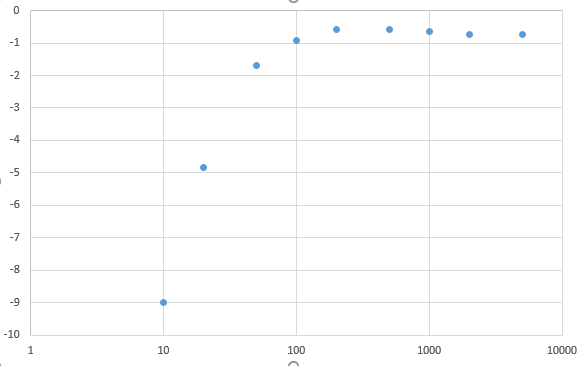
\includegraphics[width=\linewidth]{images/1_5.PNG} 
		\caption{Bode plot of summing amplifier(y:gain(dB),x:frequency(Hz))}
		\label{fig:106} 
	\end{framed}
\end{figure} 

\begin{figure}[!htbp]
	\centering 
	\begin{framed}
		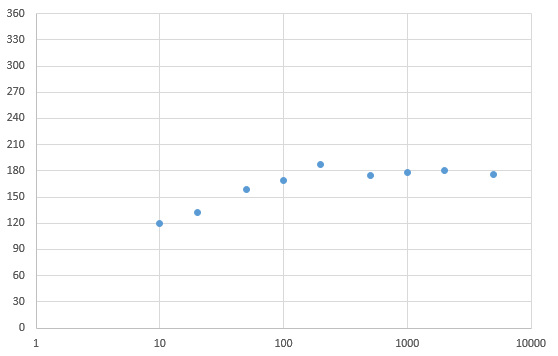
\includegraphics[width=\linewidth]{images/1_6.PNG} 
		\caption{Bode plot of summing amplifier(y:phase,x:frequency(Hz))}
		\label{fig:107} 
	\end{framed}
\end{figure}

\phantom{ } According to the gain bode plot, the circuit is a high-pass filter, because the gain goes higher while the frequency goes higher.

\phantom{ } We then set $ R_1 $ to $ 0\si{\Omega} $ and $ R_f $ to $ 50\si{\kilo\Omega} $. We also set the input signal to the proper amplitude of 300$ \si{\milli\volt} $ and frequency of $ 300\si{\hertz} $. We recorded the waveform in figure[\ref{fig:108}].
\begin{figure}[!htbp]
	\centering 
	\begin{framed}
		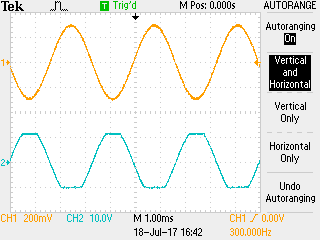
\includegraphics[width=\linewidth]{images/osc2.png}
		\caption{Waveform of the summing amplifier}
		\label{fig:108} 
	\end{framed}
\end{figure} 

\textbf{Analyze \#4:} \newline
\phantom{ } The output becomes distorted because the output amplitude reaches the resource voltage $ R_s $. The output amplitude cannot goes higher than $ R_s $, so the output waveform is flat on top and bottom. To support this reason, we recorded the following data. From table[\ref{tab:distort}], we can see that the maximum and minimum value of the output signal and $ V_{CC} $, $ V_{EE} $ are in direct proportion.
\begin{table}[!htbp]
	\centering
	\caption{The highest and lowest amplitude of output signal}
	\begin{tabular}{lcccc}
		\toprule
		No &V\_CC($ \si{\volt} $) &V\_EE($ \si{\volt} $)&V\_max($ \si{\volt} $)&V\_min($ \si{\volt} $)\\
		\midrule
		1	&+15	&-15	&+13.8	&-13.8	\\
		2	&+14	&-14	&+13.3	&-13.3	\\
		3	&+13	&-13	&+12.3	&-12.3	\\
		4	&+12	&-12	&+11.2	&-11.2	\\
		5	&+11	&-11	&+10.2	&-10.2	\\
		6	&+10	&-10	&+9.2	&-9.2	\\
		\bottomrule
	\end{tabular}
	\label{tab:distort}
\end{table}

\textbf{Analyze \#5:} \newline
\phantom{ } We applied a low frequency to $ V_1 $ and connect $ V_{out} $ to the speaker. We noticed that this low-frequency sound had a bigger volume when the capacitor is removed from the circuit. The function of the capacitor is to keep the low-frequency signals to a low gain, thus making the amplifier a high-pass filter.
